\documentclass[a4paper,10pt]{article}

% рисунки
\usepackage{graphicx}

\usepackage[T2A]{fontenc}
\usepackage[utf8]{inputenc}
\usepackage[english,russian]{babel}
\usepackage{amssymb}

\RequirePackage{caption}
\DeclareCaptionLabelSeparator{defffis}{ — }
\captionsetup{justification=centering,labelsep=defffis}

\usepackage{caption} \captionsetup[table]{labelsep=endash,justification=justified,singlelinecheck=false,font=normalsize}

\usepackage{amsmath,amsfonts,amssymb,amsthm,mathtools}

\usepackage{fancyhdr} 
\pagestyle{fancy}
\renewcommand{\headrulewidth}{0.15mm}  
\renewcommand{\footrulewidth}{0.15mm}
\lfoot{№3.4.5 Петля гистерезиса (динамический метод)}
\rfoot{\thepage}
\cfoot{}
\rhead{}
\chead{}
\lhead{Мещеряков Всеволод, Хвосточенко Константин, Б02-001}

\begin{document}
  
\begin{center}
  \section*{Лабораторная работа №3.4.5 \\Петля гистерезиса (динамический метод)\\Хвосточенко Константин и Всеволод Мещеряков, Б02-001, 28.09.2021}
\end{center}  

\vspace{5mm}
\section*{Введение}

\begin{flushleft}
  \textbf{Цель работы:} изучение петель гистерезиса раличных ферромагнитных материалов в переменных токах.

\end{flushleft}

\begin{flushleft}
  \textbf{В работе используются:} автотрансформатор, понижающий трансформатор, интегрирующая цепочка, амперметр, вольтметр, электронный осциллограф, делитель напряжения, тороидальные образцы с двумя обмотками (с сердечниками из феррита, пермаллоя и кремнистого железа).

\end{flushleft}

\section*{Теоретическая справка}

Магнитная индукция $B$ и напряжённость поля $H$ в ферромагнитном материале неоднозначно связаны между собой: индукция зависит не только от напряжённости, но и от предыстории образца. Связь между $B$ и $H$ типичного ферромагнетика иллюстрирует рисунок \ref{Theor}.

\begin{figure}[h]
	\centering
	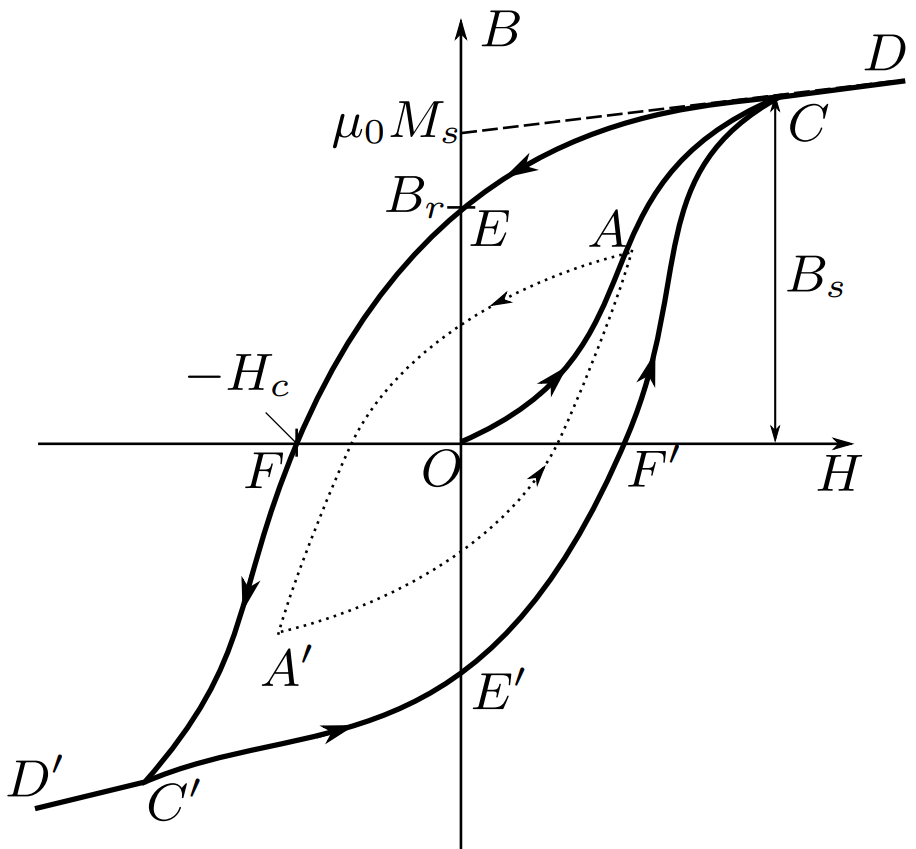
\includegraphics[scale=0.3]{lab345ris1.png}
	\caption{Петля гистерезиса ферромагнетика} \label{Theor}
\end{figure}

Если к ферромагнитному образцу прикладывать переменное внешнее магнитное поле, то его состояние на плоскости $H-B$ будет изменяться по замкнутой кривой -- \textit{петле гистерезиса}. Резмер петли определяется максимальным значением напряжённости $H$ в цикле (например, петля $AA'$, обозначенная пунктиром на рисунке \ref{Theor}). Если амплитуда напряжённости достаточно велика, то образец будет периодически достигать \textit{насыщения}, что на рисунке соответствует кривой $CERC'E'F'C$ (\textit{предельная петля гистерезиса}). Пересечение предельной петли с вертикальной осью соответствует остаточной индукции $B_r$, пересечение с горизонтальной осью -- коэрцитивному полю $H_c$. Крайние точки петель, соответствующие амплитудным значениям $H$ (например, точка $A$ на рисунке \ref{Theor}), лежат на \textit{начальной кривой намагничивания} ($OAC$).

\textbf{Измерение магнитной индукции.} Магнитную индукцию $B$ удобно определять с помощью ЭДС, возникающей при измерении магнитного потока $\Phi$ в катушке, намотанной на образец. Пусть катушка с $N$ витками плотно охватывает образец сечением $S$, и индукция $B$ в образце однородна. Тогда\[\left|B\right|=\frac{1}{SN}\int\varepsilon\text{d}t.\]Таким образом, для определения $B$ нужно проинтегрировать сигнал, наведённый меняющимся магнитным полем в измерительной катушке, намотанной на образец.

Для интегрирования в работе используется \textit{интегрирующая} $RC$-цепочка. Входное напряжение от источника $U_{\text{вх}}(t)$ подаётся на последовательно соединённые резистор $R_{\text{и}}$ и конденсатор $C_{\text{и}}$. Выходное напряжение $U_{\text{вых}}(t)$ снимается с конденсатора. Предположим, что (1) сопротивление источника мало по сравнению с $R_{\text{и}}$; (2) выходное сопротивление (сопротивление на входе осциллографа), напротив, велико: $R_{\text{вых}}\gg R_{\text{и}}$; и, наконец, (3) сопротивление $R_{\text{и}}$ достаточно велико, так что почти всё падение напряжения приходится на него, а $U_{\text{вых}}\ll U_{\text{вх}}$. В таком случае ток цепи равен $I=\frac{U_{\text{вх}}-U_{\text{вых}}}{R_{\text{и}}}\approx\frac{U_{\text{вх}}}{R_{\text{и}}}$, и входное и выходное сопротивление связаны соотношением\[U_{\text{вых}}\frac{q}{C_{\text{и}}}=\frac{1}{C_{\text{и}}}\int_0^tI\text{d}t\approx\frac{1}{\tau_{\text{и}}}\int_0^tU_{\text{вх}}\text{d}t,\]где $\tau_{\text{и}}=R_{\text{и}}C_{\text{и}}$ -- постоянная времени $RC$-цепочки. Для индукции поля получаем\[\left|B\right|=\frac{1}{SN}\int U_{\text{вх}}\text{d}t=\frac{\tau_{\text{и}}}{SN}U_{\text{вх}}.\]



\section*{Экспериментальная установка}

Схема установки приведена на рисунке \ref{Device}. Напряжение сети (220 Вт, 50 Гц) с помощью регулировочного автотрансформатора Ат через разделительный понижающий трансформатор Тр подаётся на намагничивающую обмотку $N_0$ исследуемого образца.

\begin{figure}[h!]
	\centering
	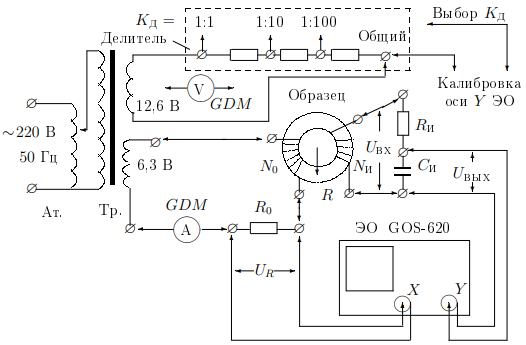
\includegraphics[scale=0.8]{lab345ris2.png}
	\caption{Схема установки для исследования намагничивания образцов} \label{Device}
\end{figure}

Действующее значение переменного тока в обмотке $N_0$ измеряется амперметром $A$ (мультиметром GDM). Последовательно с амперметром включено сопротивление $R_0$, напряжение с которого подаётся на вход $X$ электронного осциллографа (ЭО). Это напряжение пропорционально току в обмотке $N_0$, а следовательно и напряжённости $H$ магнитного поля в образце.

Для измерения магнитной индукции $B$ с измерительной обмотки $N_{\text{и}}$ на вход интегрирующей $RC$-цепочки подаётся напряжение $U_{\text{и}}$ ($U_{\text{вх}}$), пропорциональное производной $\dot{B}$, а с выхода снимается напряжение $U_C$ ($U_{\text{вых}}$), пропорциональное величине $B$, и подаётся на вход $Y$ осциллографа.

Замкнутая кривая, возникающая на экране, воспроизводит в некотором масштабе (различном для осей $X$ и $Y$) петлю гистерезиса. Чтобы придать этой кривой количественный смысл, необходимо установить масштабы изображения, т.е. провести калибровку каналов $X$ и $Y$ ЭО. Для этого, во-первых, надо узнать, каким напряжениям (или токам) соответствуют амплитуды сигналов, видимых на экране, и во-вторых, -- каким значениям $B$ и $H$ соответствуют эти напряжения (или токи).

\textbf{Измерения напряжения с помощью осциллографа.} Исследуемый сигнал подаётся на вход $X$: длина $2x$ горизонтальной черты, наблюдаемой на экране, характризует удвоенную амплитуду сигнала.

Если известна чувствительность усилителя $K_X$ в вольтах на деление шкалы экрана, то удвоенная амплитуда напряжения определяется произведением\[2U_{X,0}=2x\cdot K_X.\]Напряжение, подаваемое на ось $Y$, измеряется аналогично.

Калибровку осей осциллографа ($K_X$ и $K_Y$) можно использовать для построения кривой гистерезиса в координатах $B$ и $H$: зная величину сопротивления $R_0$, с которого снимается сигнал, можно определить чувствительность канала по току $K_{XI}=\frac{K_X}{R_0}\ \left[\frac{\text{А}}{\text{дел}}\right]$ и затем определить цену деления шкалы в $\frac{\text{А}}{\text{м}}$.

Зная чувствительность $K_Y$, можно рассчитать цену деления вертикальной шкалы ЭО в теслах.

Наличие в схеме амперметра и вольтметра позволяет провести \textit{независимую калибровку} усилителей ЭО, т.е. проверить значения коэффициентов $K_X$ и $K_Y$ (ручки регулировки усиления ЭО могут быть сбиты).

\textbf{Проверка калибровки горизонтальной оси ЭО с помощью амперметра} проводится при закороченной обмотке $N_0$. Эта обмотка с помещённым в неё ферромагнитным образцом являеся нелинейным элементом, так что ток в ней не имеет синусоидальной формы, и это не позволяет связать амплитуду тока с показаниями амперметра.

При закороченной обмотке $N_0$ амперметр $A$ измеряет эффективное значение синусоидального тока $I_{\text{эф}}$, текущего через известное сопротивление $R_0$. Сигнал с этого сопротивления подаётся на вход $X$ ЭО. Измерив $2x$ -- длину горизонтальной прямой на экране, можно рассчитать $m_X$ -- чувствительность канала $X$:\[m_X=\frac{2\sqrt2R_0I_{\text{эф}}}{2x}\quad\left[\frac{\text{В}}{\text{дел}}\right].\]

\textbf{Проверка калибровки вертикальной оси ЭО с помощью вольтметра.} Сигнал с обмотки 12,6 В понижающего трансформатора (\ref{Device}) подаётся на делитель напряжения. Часть этого напряжения снимается с делителя с коэффициентом деления $K_{\text{д}}$ ($\frac{1}{10}$ или $\frac{1}{100}$) и подаётся на вход $Y$ ЭО (вместо напряжения $U_C$). Мультиметр $V$ измеряет напряжение $U_{\text{эф}}$ на этих же клеммах делителя. Измерив $2y$ -- длину вертикальной прямой на экране, можно рассчитать чувствительность канала $Y$:\[m_Y=\frac{2\sqrt2R_0U_{\text{эф}}}{2x}\quad\left[\frac{\text{В}}{\text{дел}}\right].\]

При этом тороид должен быть отключен, так как несинусоидальный ток нагрузки в первичной обмотке тороида приводит к искажению формы кривой напряжения и на обмотке трансформатора, питающей делитель.

\textbf{Постоянную времени RC-цепочки} можно определить экспериментально. С обмотки 6,3 В на вход интегрирующей цепочки подаётся синусоидальное напряжения $U_{\text{вх}}$. На вход $Y$ осциллографа поочерёдно подаются сигналы со входа ($U_{\text{вх}}$) и выхода ($U_{\text{вых}}$) $RC$-цепочки. Измерив амплитуды этих сигналов с помощью осциллографа, можно рассчитать постоянную времени $\tau=RC$. Тогда\[RC=\frac{U_{\text{вх}}}{\Omega U_{\text{вых}}}.\]

\section*{Ход работы}

\subsection*{I. Петля гистерезиса на экране ЭО}
Перед началом работы запишем необходимую информацию о каждом исследуемом образце в таблицу \ref{data}.

\begin{table}[h!]
	\centering
	\caption{Параметры исследуемых образцов} \label{data}
	\begin{tabular}{|l|l|l|l|l|}
		\hline
		Название материала образца & $N_0$ & $N_u$ & $S \text{ см}^2$  & $2\pi R$ см \\ \hline
		Кремнистое железо          & 35 & 350 & 1,2 & 10 \\ \hline
		Феррит                     & 35 & 400 & 3,0 & 25 \\ \hline
		Пермалой                   & 40 & 200 & 3,8 & 24 \\ \hline
	\end{tabular}
\end{table}


Теперь соберём схему согласно рисунку \ref{Device} и подготовим приборы к работе. Подберём ток питания в намагничивающей обмотке и коэффициенты усиления ЭО так, чтобы предельная петля гистерезиса занимала большую часть экрана. Получив предельную петлю, уменьшим ток до исчезновения горизонтальных "усов". Отцентруем вертикальный и горизонтальный лучи.

Для каждого образца сделаем фотографию предельной петли. Сфотографируем кривую при ещё двух различных значениях тока при его уменьшении, и полученные оттуда координаты концов частных петель используем для проведения кривой. Эта кривая будет проходить в непосредственной близости от начальной кривой намагничивания. Кривая намагничивания и предельная петля для каждого из образцов показаны на рисунках \ref{Loop_1}, \ref{Loop_2} и \ref{Loop_3}. 

\begin{figure}[h!]
	\centering
	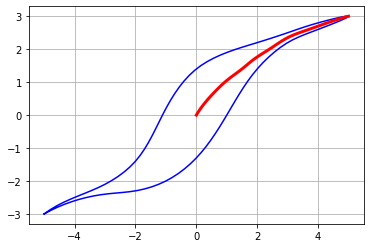
\includegraphics[scale=0.8]{lab345ris3.png}
	\caption{Предельная петля гистерезиса и начальная кривая намагничивания для образца из кремнистого железа} \label{Loop_1}
\end{figure}

\begin{figure}[h!]
	\centering
	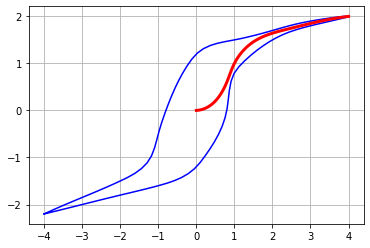
\includegraphics[scale=0.8]{lab345ris4.png}
	\caption{Предельная петля гистерезиса и начальная кривая намагничивания для образца из феррита} \label{Loop_2}
\end{figure}

\begin{figure}[h!]
	\centering
	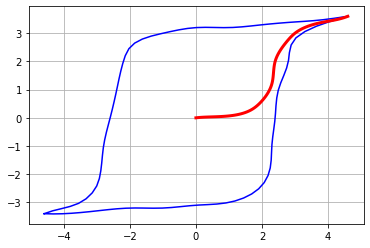
\includegraphics[scale=0.8]{lab345ris5.png}
	\caption{Предельная петля гистерезиса и начальная кривая намагничивания для образца из пермаллоя} \label{Loop_3}
\end{figure}

Рассчитаем цену деления ЭО для петли в $\frac{\text{А}}{\text{м}}$ для оси $X$ по формуле\[H=\frac{N_0K_X}{2\pi RR_0}\]и в $\text{Тл}$ для оси $Y$ \[B=\frac{R_{\text{и}}C_{\text{и}}K_Y}{SN_{\text{и}}}.\]Измерим по предельной петле двойные амплитуды для коэрцитивной силы $\left[2x\left(c\right)\right]$ и индукции насыщения $\left[2y\left(s\right)\right]$. Данные значения вместе с коэффициентами усиления $K_x$ и $K_y$, током $I_{\text{эф}}$ и ценами деления $H$ и $B$ занесем в таблицу \ref{data1}.
Будем считать, что погрешность определения $2x$ и $2y$ равна 1 делению.

\begin{table}[h!]
	\centering
	\caption{Измеренные данные} \label{data1}
	\begin{tabular}{|l|l|l|l|l|l|l|l|}
		\hline
		Название материала образца & $K_x, \frac{\text{мВ}}{\text{дел}}$  & $K_y,\frac{\text{мВ}}{\text{дел}}$ & $2x$, дел & $2y$, дел & $I_{\text{эф}}$ А & $H,\ \frac{\text{А}}{\text{м}}$ & $B$, Тл \\ \hline
		Кремнистое железо          & 50 & 50 & 50 & 30 & 0,620 & 58,33 & 0,476 \\ \hline
		Феррит                     & 20 & 20 & 40 & 20 & 0,208 & 9,33 & 0,067 \\ \hline
		Пермалой                   & 20 & 50 & 40 & 32 & 0,677 & 11,11 & 0,263 \\ \hline
	\end{tabular}
\end{table}

Отсюда и из начальной кривой намагничивания можно найти коэрцитивное поле $H_c$ и намагниченность насыщения $B_s$. Результаты вычисления для каждого образца b их справочные значения приведены в таблице \ref{data5}.

\begin{table}[h!]
	\centering
	\caption{Проверка калибровки оси $X$} \label{data5}
\begin{tabular}{|l|l|l|l|l|}
	\hline
	Название материала образца & $H_c,\frac{\text{А}}{\text{м}}$ & $B_s,$ Тл & $H_0,\frac{\text{А}}{\text{м}}$ & $B_0$, Тл \\ \hline
	Кремнистое железо          & 64$\pm$6 & 0,67$\pm$0,05 & 32--72\cite{g}   &  $\leq$ 1\\ \hline
	Феррит                     & 7,5$\pm$0,9 & 0,080$\pm$0,007 & 1,2--16\cite{a}  & 0,05--0,4 \\ \hline
	Пермалой                   & 26,7$\pm$1,1 & 0,82$\pm$0,03 & 8--80 \cite{f}  & 0,73--0,85 \\ \hline
\end{tabular}
\end{table}


\subsection*{II. Проверка калибровки оси $X$ ЭО с помощью амперметра}

Отключим намагничивающую обмотку $N_0$ от цепи, соединив оба провода, идущих к обмотке, на одной из её клемм. С помощью автотрансформатора подберём такой ток через сопротивление $R_0$, при котором горизонтальная прямая занимает большую часть экрана ЭО. Вычислим $m_x$ для каждого $K_x$. Результаты занесем в таблицу \ref{data2}

\begin{table}[h!]
	\centering
	\caption{Проверка калибровки оси $X$} \label{data2}
	\begin{tabular}{|l|l|l|l|}
		\hline
		           & $I_{\text{эф}}$, мА & $2x$, дел & $m_x~\frac{\text{мВ}}{\text{дел}}$ \\ \hline
		$K_x = 20~\frac{\text{мВ}}{\text{дел}}$  & 186,1 $\pm 0,5$ & 8,2 $\pm$0,2 & 19,3 $\pm$ 0,5 \\ \hline
		$K_x = 50~\frac{\text{мВ}}{\text{дел}}$  & 508 $\pm$ 5 & 8,6$\pm$0,2  & 50,1$\pm$ 1,3 \\ \hline
	\end{tabular}
\end{table}

\subsection*{III. Проверка калибровки оси $Y$ ЭО с помощью вольтметра}

Соединим вход $Y$ ЭО с клеммами делителя "$\frac{1}{100}$--земля". Не меняя рабочего коэффициента $K_Y$, подберём с помощью автотрансформатора напряжение, при котором вертикальная прямая занимает почти весь экран. Подключим вольтметр $V$ к тем же точкам делителя и измерим эффективное значение напряжения. Затем расчитаем $m_y$ для каждого $K_y$. Результаты представим в таблице  \ref{data3}.

\begin{table}[h!]
	\centering
	\caption{Проверка калибровки оси $Y$} \label{data3}
	\begin{tabular}{|l|l|l|l|}
		\hline
		& $U_{\text{эф}}$, мВ & $2y$, дел & $m_y~\frac{\text{мВ}}{\text{дел}}$ \\ \hline
		$K_y = 20~\frac{\text{мВ}}{\text{дел}}$  & 40 $\pm 0,1$ & 6 $\pm$0,2 & 18,9 $\pm$ 0,6 \\ \hline
		$K_y = 50~\frac{\text{мВ}}{\text{дел}}$  & 98,5 $\pm 0,4$  & 6$\pm$0,2 & 46,4 $\pm$ 1,6 \\ \hline
	\end{tabular}
\end{table}

\subsection*{IV. Определение $\tau$ -- постоянной времени $RC$-цепочки}

Для определения напряжений на входе и выходе интегрирующей ячейки соединим вход ячейки с обмоткой 6,3 В трансформатора. Подключим $Y$-вход ЭО ко входу интегрирующей ячейки и отключим $X$-вход ЭО. Установим чувствительность $K_Y=2~\frac{\text{В}}{\text{дел}}$ и подберём с помощью автотрансформатора такой ток, при котором вертикальная прямая занимает большую часть экрана, и определим входное напряжение на $RC$-цепочке как $U_{\text{вх}}=2y\cdot K_Y=\left(13,6\pm0,4\right)~\text{В}$ (считаем, что погрешность определения $2y$ равна 0,2 дел).

Теперь, не изменяя тока, переключим $Y$-вход ЭО к выходу ячейки (конденсатору $C$), установим $K_Y=20,0~\frac{\text{мВ}}{\text{дел}}$ и аналогичным образом определим напряжение $U_{\text{вых}}=\left(104\pm4\right)~\text{мВ}$.

Расчитаем постоянную времени $\tau = \frac{U_{\text{вх}}}{\Omega U_{\text{вых}}} = 0,416 \pm 0,020$ с. Ту же величину найдем с помощью значений $R = 20$кОм и $C$мкФ, указанных на установке, $\tau = 0,4$ с. Видно, что в пределах погрешности данные результаты совпадают.

Также выполнено условие того, что $R\gg\frac{1}{\Omega C}$, так как $R=20,0~\text{кОм}$, а $\frac{1}{\Omega C}=159,2$ КОм.

\section*{Вывод}


В данной работе были изучены петли гистерезиса различных ферромагнитных материалов в переменных токах.

В первой части работы были получены предельные петли и начальные кривые намагничивания для образцов из пермаллоя, феррита и кремнистого железа. Были рассчитаны цены деления ЭО для петель в $\frac{\text{А}}{\text{м}}$ для оси $X$ и в $\text{Тл}$ для оси $Y$, откуда были найдены коэрцитивная сила $H_c$, индукция насыщения $B_s$. Измеренные значения в пределах погрешности совпали со справочными.

Во второй и третьей частях работы была проведена проверка калибровок осей ЭО с помощью вольтметра и амперметра. Для рабочих коэффициентов $K_X$ и $K_Y$  были получены значения чувствительности каналов $m_X$ и $m_Y$ соответственно. Для $K_x = 50 ~\frac{\text{мВ}}{\text{дел}}$  $m_x$ в пределах погрешности совпало с ним. Для остальных коэффициентов $K_x$ и $K_y$ значения не попали в пределы погрешности, однако отклонение оказалоссь малым (максимальное отклонение от нижной границы погрешности не превысило 4$\%$).

В последней части работы  была экспериментально проверена постоянная времени интегрирующей цепочки, которая получилась равной $\tau=\left(0,416\pm0,020\right)~\text{с}$, т.е. в пределах погрешности совпадающей с $\tau=0,4~\text{с}$, рассчитанной по указанным на установке величинам. Также было подтверждено условие применимости приближений, в которых работает $RC$-цепочка. 
\begin{thebibliography}{3}
	
	\bibitem{g}
	 M. A. Akhter-D. J. Mapps-Y. Q. Ma Tan-Amanda Petford-Long-R. Doole; Mapps; Ma Tan; Petford-Long; Doole (1997). “Thickness and grain-size dependence of the coercivity in permalloy thin films”. Journal of Applied Physics. 81 (8): 4122.
	 
	\bibitem{a}
	Zhenghong Qian; Geng Wang; Sivertsen, J.M.; Judy, J.H. (1997). “Ni Zn ferrite thin films prepared by Facing Target Sputtering”. IEEE Transactions on Magnetics. 33 (5): 3748—3750.
	
	\bibitem{f}
	M. A. Akhter-D. J. Mapps-Y. Q. Ma Tan-Amanda Petford-Long-R. Doole; Mapps; Ma Tan; Petford-Long; Doole (1997). “Thickness and grain-size dependence of the coercivity in permalloy thin films”. Journal of Applied Physics. 81 (8): 4122. 
	
\end{thebibliography} 

\end{document}